 %\documentclass[wcp,gray]{jmlr} % test grayscale version
\documentclass[wcp]{jmlr}

 % The following packages will be automatically loaded:
 % amsmath, amssymb, natbib, graphicx, url, algorithm2e

 %\usepackage{rotating}% for sideways figures and tables
\usepackage{longtable}% for long tables

 % The booktabs package is used by this sample document
 % (it provides \toprule, \midrule and \bottomrule).
 % Remove the next line if you don't require it.
\usepackage{booktabs}
 % The siunitx package is used by this sample document
 % to align numbers in a column by their decimal point.
 % Remove the next line if you don't require it.
%\usepackage[load-configurations=version-1]{siunitx} % newer version
%\usepackage{siunitx}

 % change the arguments, as appropriate, in the following:
\jmlrvolume{1}
\jmlryear{2014}
\jmlrworkshop{ICML 2014 AutoML Workshop}

\title[Hyperopt-Sklearn]{Hyperopt-Sklearn: Subtitle?}

 % Use \Name{Author Name} to specify the name.
 % If the surname contains spaces, enclose the surname
 % in braces, e.g. \Name{John {Smith Jones}} similarly
 % if the name has a "von" part, e.g \Name{Jane {de Winter}}.
 % If the first letter in the forenames is a diacritic
 % enclose the diacritic in braces, e.g. \Name{{\'E}louise Smith}
%\nametag{\thanks{Affiliation: D\'epartement d'Informatique et Recherche Op\'erationel, Universit\'e de Montr\'eal}}
% \nametag{\thanks{Corresponding author}}
 % Two authors with the same address
  \author{
      \\
      \Name{Brent Komer} \Email{brent.komer@uwaterloo.ca}\\
      \Name{James Bergstra} \Email{james.bergstra@uwaterloo.ca}\\
      \Name{Chris Eliasmith} \Email{celiasmith@uwaterloo.ca}\\
      \addr Centre for Theoretical Neuroscience\\University of Waterloo\\
  }


%\editor{Editor's name XXX}
 % \editors{List of editors' names}

\iffalse   % UNCOMMENT THIS STUFF TO BE MORE SPACE EFFICIENT
\renewcommand\floatpagefraction{.9}
\renewcommand\dblfloatpagefraction{.9} % for two column documents
\renewcommand\topfraction{.9}
\renewcommand\dbltopfraction{.9} % for two column documents
\renewcommand\bottomfraction{.9}
\renewcommand\textfraction{.1}
\setcounter{totalnumber}{50}
\setcounter{topnumber}{50}
\setcounter{bottomnumber}{50}
\fi

\begin{document}

\maketitle

\begin{abstract}
    Hyperopt-sklearn is a new software project that provides automatic algorithm configuration of the Scikit-learn machine learning library.
    Following Auto-Weka, we take the view that the choice of classifier and even the choice of pre-processing module can be taken together to represent a {\em single large hyperparameter optimization problem}.
    We use Hyperopt to define a search space that encompasses many standard components (e.g. SVM, RF, KNN, PCA, TFIDF) and common patterns of composing them together.
    We demonstrate, using search algorithms in Hyperopt and standard benchmarking data sets (MNIST, 20-Newsgroups, Convex Images), that searching this space is practical and effective.
    In particular, we improve on best-known scores for the model space for both MNIST and Convex Images.
\end{abstract}
%\begin{keywords}
%Bayesian Optimization, Model Selection, Hyperparameter Optimization, Scikit-learn
%\end{keywords}

\section{Introduction}
\label{sec:intro}

The size of data sets and the speed of computers have increased to the point where it is often easier to fit complex functions to data using statistical estimation techniques than it is to design them by hand.
The fitting of such functions (training machine learning algorithms) remains a relatively arcane art, typically mastered in the course of a graduate degree and years of experience.
Recently however, techniques for automatic algorithm configuration based on
Regression Trees~\citep{hutter+hoos+leyton-brown:2011},
Gaussian Processes~\citep{MoTiZi78,snoek+larochelle+adams:2012nips},
and density-estimation techniques~\citep{bergstra+bardenet+bengio+kegl:2011}
have emerged as viable alternatives to hand-tuning by domain specialists.

Hyperparameter optimization in machine learning systems was first applied to neural networks and convnets, where the number of parameters can be overwhelming:
for example \citet{bergstra+bardenet+bengio+kegl:2011} tuned Deep Belief Networks with up to 32 hyperparameters,
and \citet{bergstra+yamins+cox:2013} showed that similar methods could be useful even in a convnet model with 238 hyperparameters.
Relative to DBNs and convnets, algorithms such as RBF-SVMs and Random Forests (RFs) have a small-enough number of hyperparameters that manual tuning and grid or random search provides satisfactory results.

Taking a step back though, there is often no particular reason to use either an RBF-SVM or an RF when they are both computationally viable.
A model-agnostic practitioner may simply prefer to go with the one that provides greater accuracy.
In this light, {\em the choice of classifier can be seen as hyperparameter} alongside the $C$-value in the SVM and the max-tree-depth of the RF.
Indeed the choice and configuration of {\em pre-processing} components may likewise be seen as part of the model selection / hyperparameter optimization problem.
The Auto-Weka project \citep{thornton+hutter+hoos+leyton-brown:2012} was the first to show that an entire library of machine learning approaches (Weka~\citep{hall2009weka}) can be searched within the scope of a single run of hyperparameter tuning.
However, Weka is a GPL-licensed Java library, and was not written with scalability in mind. These factors limit the utility of Auto-Weka.
Scikit-learn~\citep{sklearn} is another library of machine learning algorithms that is written in Python with many modules in C for greater speed, and is BSD-licensed.
Scikit-learn is widely used in the scientific Python community and supports many machine learning application areas.

Our goal in this paper is to introduce Hyperopt-Sklearn -- a project that brings the benefits of automatic algorithm configuration to users of Python and scikit-learn.
Hyperopt-Sklearn uses Hyperopt~\citep{hyperopt} to describe a search space over possible configurations of Scikit-Learn components, including pre-processing and classification modules.
Section 2 describes our configuration space of 7 classifiers and 4 preprocessing modules that encompasses a strong set of classification systems for dense and sparse feature classification (of images and text).
Section 3 presents experimental evidence that search over this space is viable, meaningful, and effective.
Section 4 presents a discussion of the results, and directions for future work.


\section{Searching Scikit-learn with Hyperopt}

The configuration space we experiment on below includes five preprocessing algorithms and seven classification algorithms.
The full search space is illustrated in Figure~\ref{fig:searchspace}.
The preprocessing algorithms were (by class name, followed by n. hyperparameters + n. unused hyperparameters): \texttt{PCA}(2), \texttt{StandardScaler}(2), \texttt{MinMaxScaler}(1), \texttt{Normalizer}(1), and \texttt{TF-IDF}(0+9).
The first four preprocessing algorithms were for dense features.
PCA performed whitening or non-whitening principle components analysis.
The \texttt{StandardScaler}, \texttt{MinMaxScaler}, and \texttt{Normalizer} did various feature-wise affine transforms to map numeric input features onto values near 0 and with roughly unit variance.
The \texttt{TF-IDF} pre-processing module performed feature extraction from text data.
The classification algorithms were (by class name (used + unused hyperparameters)): \texttt{SVC}(23), \texttt{LinearSVC}(6), \texttt{KNN}(4+5), \texttt{RandomForest}(8), \texttt{ExtraTrees}(8), \texttt{SGD}(8+4), and \texttt{MultinomialNB}(2).
The \texttt{SVC} module is a fork of LibSVM, and our wrapper has 23 hyperparameters because we treated each possible kernel as a different classifier, with its own set of hyperparameters: Linear(4), RBF(5), Polynomial(7), and Sigmoid(6).

In total, our parameterization had 65 hyperparameters: 6 for preprocessing and 59 for classification.
How many boolean: 15
How many categorical: 14
How many discrete: 17
How many real-valued: 19
It is important to note that although the total number of hyperparameters is large, the number of {\em active} hyperparameters describing any one model is much smaller: a model consisting of \texttt{PCA} and a \texttt{RandomForest} for example,
would have only 12 active hyperparameters (1 for the choice of preprocessing, 2 internal to PCA, 1 for the choice of classifier and 8 internal to the RF).
Hyperopt description language allows us to differentiate between {\em conditional} hyperparameters (which must always be assigned) and {\em non-conditional} hyperparameters (which may remain unassigned when they would be unused).
We make use of this mechanism extensively so that Hyperopt's search algorithms do not waste time learning by trial and error that e.g. RF hyperparameters have no effect on SVM performance.
Even within a single classifier, there were instances of conditional parameters: \texttt{KNN} has conditional parameters depending on the distance metric,
and \texttt{LinearSVC} has 3 binary parameters (``loss'', ``penalty'', and ``dual'') that admit only 4 valid joint assignments.
We also included a blacklist of (preprocessing, classifier) pairs that did not work together, e.g. PCA and MinMaxScaler were incompatible with MultinomialNB, TF-IDF could only be used for text data, and the tree-based classifiers were not
compatible with the sparse features produced by the TF-IDF preprocessor.
Allowing for a 10-way discretization of real-valued hyperparameters, and taking these conditional hyperparameters into account, a grid search of our search space would still require an infeasible number of evalutions (on the order of $10^{12}$).

Following Scikit-learn's convention, hyperopt-sklearn provides an \texttt{Estimator} class with a \texttt{fit} method and a \texttt{predict} method.
The \texttt{fit} method of this class performs hyperparameter optimization, and after it has completed, the \texttt{predict} method applies the best model to test data.
Hyperopt makes it possible to parallelize the model search over a cluster, with communication handled via a MongoDB instance.
Each evaluation during optimization performs training on a large fraction of the training set, estimates test set accuracy on a validation set, and returns that validation set score to the optimizer.
At the end of search, the best configuration is retrained on the whole data set to produce the classifier that handles subsequent \texttt{predict} calls.


\section{Experiments}
We conducted experiments on three data sets to establish that hyperopt-sklearn can find accurate models on a range of data sets
hyperopt-sklearn finds accurate models,
%(b) different data sets lead hyperopt-sklearn to select different models, and
(c) search can be carried out in a reasonable amount of time.
Results were collected on three data sets: MNIST, 20-Newsgroups, and Convex Images.
MNIST~\citep{lecun+bottou+bengio+haffner:1998} is a well-known data set of 70K $28\times 28$ greyscale images of hand-drawn digits.
20-Newsgroups is a 20-way classification data set of 20000 newsgroup messages (\citet{20newsgroups}, we did not remove the headers for our experiments).
Convex Images~\citep{larochelle+etal:2007} is a binary classification task of distinguishing pictures of convex white-colored regions in small ($32\times 32$) black-and-white images.

To establish that searching the full space is effective,
we performed optimization runs of up to 300 function evaluations searching either the entire space, or else subspaces that corresponded to specific classifier types.
We used three optimization algorithms in Hyperopt: random search, annealing, and TPE.
Figure~\ref{fig:avg_test_scores} shows that the performance of the model found from throughout the entire search space was not statistically inferior to the best model pulled from each classifier subspace;
there was no penalty for keeping all options open during search.
Table~\ref{tbl:acc} lists the test set scores of the best models found by cross-validation, as well as some points of reference from previous work.
Hyperopt-sklearn's scores are relatively good on each data set, indicating that with hyperopt-sklearn's parameterization, Hyperopt's optimization algorithms are competitive with human experts.
\citep{eggensperger+etal:2013}
\citep{scipy}.

\begin{table}
    \caption{
        Hyperopt-sklearn scores relative to selections from literature on the three data sets used in our experiments.
        On MNIST, hyperopt-sklearn is one of the best-scoring methods that does not use image-specific domain knowledge (these scores and others may be found at http://yann.lecun.com/exdb/mnist/).
        On 20 Newsgroups, XXX.
        On Convex Images, hyperopt-sklearn outperforms previous automatic algorithm configuration approaches~\citep{eggensperger+etal:2013} and manual tuning~\citep{larochelle+etal:2007}.
    }
    \label{tbl:acc}
    \centering
    \small
    \begin{tabular}{llllll}
        \hline
        \multicolumn{2}{c}{\textbf{MNIST}} & \multicolumn{2}{c}{\textbf{20 Newsgroups}} & \multicolumn{2}{c}{\textbf{Convex Images}}  \\
        Approach & Accuracy  & Approach & F-Score & Approach & Accuracy\\
        \hline
        Committee of convnets & 99.8\%                & CFC & .928 & \textbf{hyperopt-sklearn} & 88.7\%\\
	\textbf{hyperopt-sklearn} & \textbf{98.7}\%   & hyperopt-sklearn & \textbf{.856} & hp-dbnet & 84.6\% \\
        libSVM grid search & 98.6\%                   & SVMTorch & .848 & dbn-3 & 81.4\%\\
        Boosted trees & 98.5\%                        & LibSVM & .843 &  &  \\
    \end{tabular}
\end{table}

%To support the hypothesis that the search carried out by hyperopt-sklearn is necessary for good performance on a range of data sets, we present three pieces of evidence.
%First, looking again at Figure~\ref{fig:avg_test_scores}, note that 
%Figure~\ref{fig:pies} shows that 
%different data sets lead hyperopt-sklearn to select

\begin{figure}
    \centering
    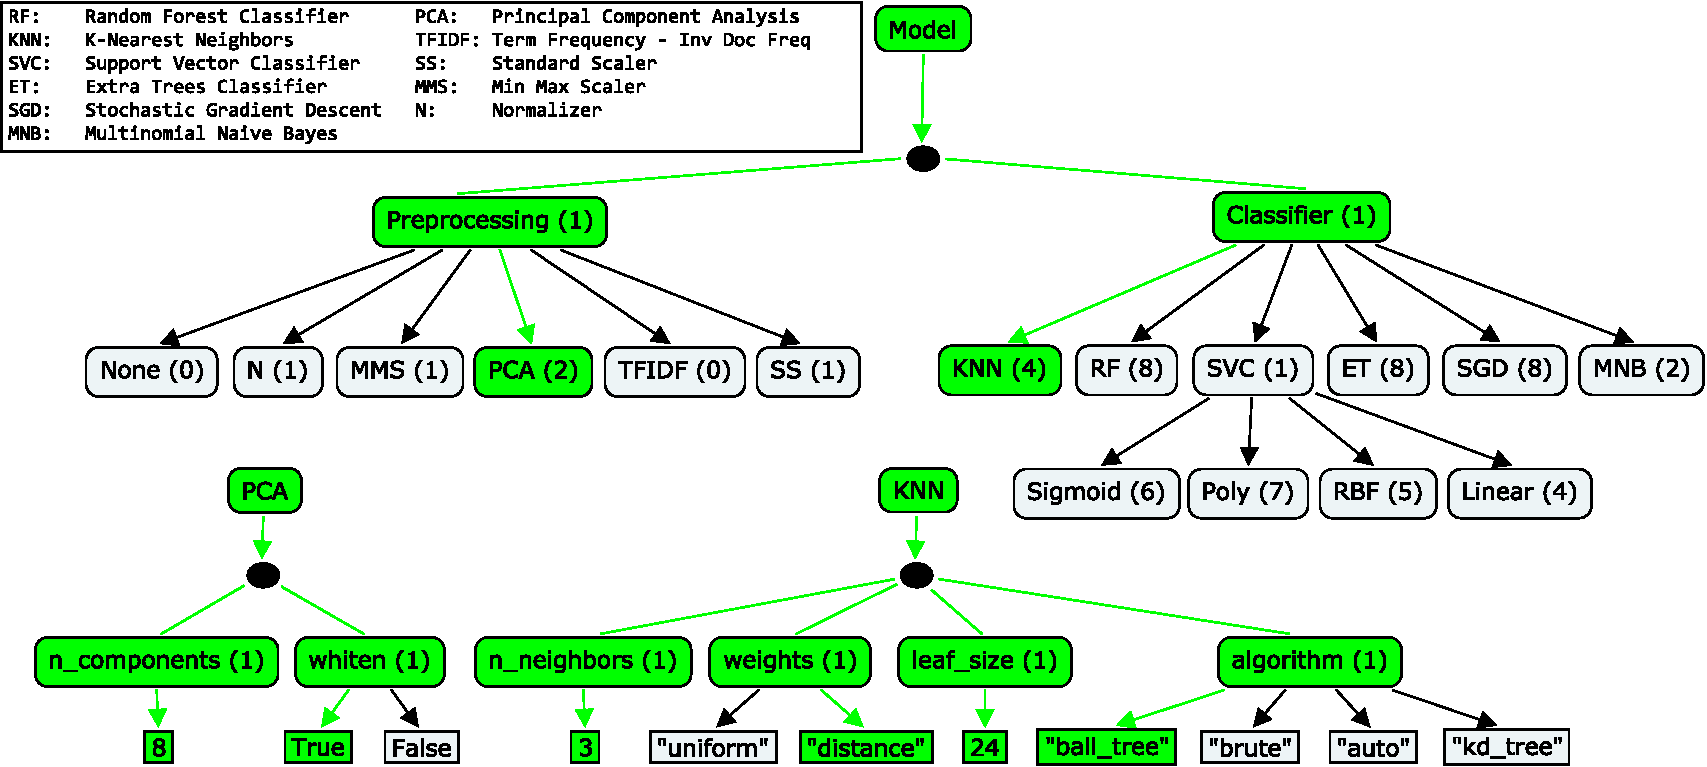
\includegraphics[width=\textwidth]{graphics/sklearn_space_all_together}
    \caption{
	    XXX
    }
    \label{fig:space}
\end{figure}
\begin{figure}
    \centering
    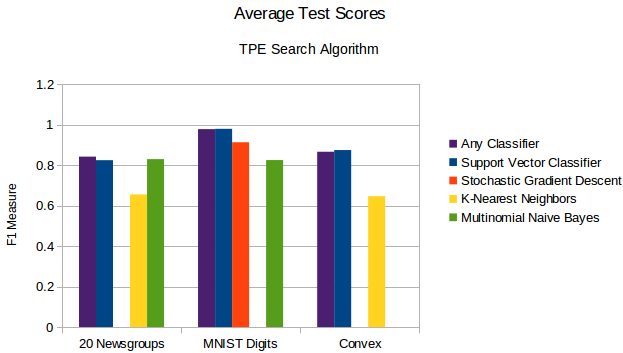
\includegraphics[width=2.90in]{graphics/AverageTestScoresClassifiersTPE}
    \caption{
        For each data set, searching the full configuration space (``Any Classifier'') delivered performance approximately on par with a search that was restricted to the best classifier type.
        (Best viewed in color.)
    }
    \label{fig:avg_test_scores}
%\vspace{-3em}
\end{figure}

\begin{figure}
    \centering
    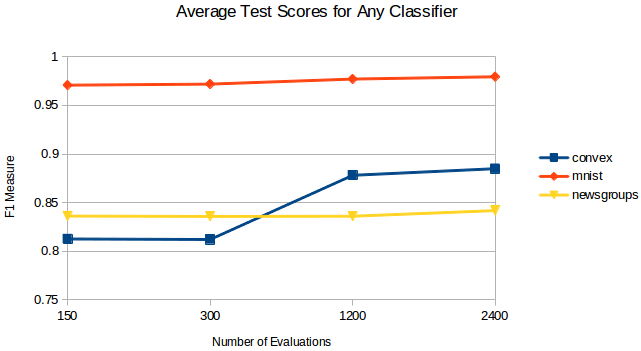
\includegraphics[width=\textwidth]{graphics/scores_by_classifier}
    \caption{
	    XXX
    }
    \label{fig:per_clf}
\end{figure}


\begin{figure}
    \centering
    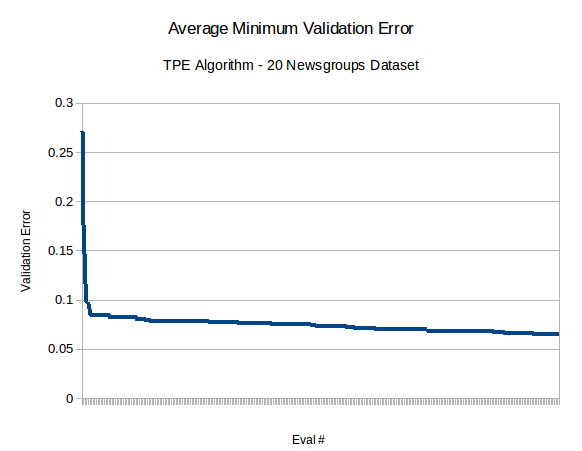
\includegraphics[width=\textwidth]{graphics/AvgMinValidErrorTPE}
    \caption{
	    XXX
    }
    \label{fig:errtpe}
\end{figure}

\begin{figure}
    \centering
    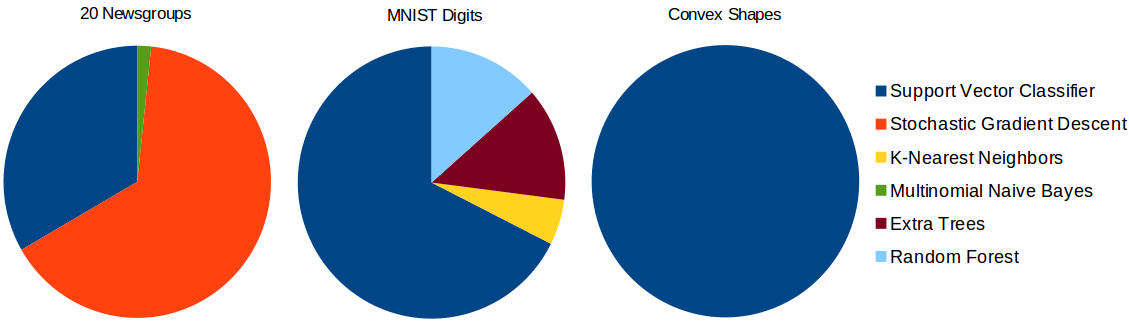
\includegraphics[width=\textwidth]{graphics/pie}
    \caption{
	    XXX
    }
    \label{fig:npie}
\end{figure}



\section{Discussion and Future Work}
Future Work
Lots of areas for future work:
Speed: Aborting points early when using K-fold validation
Applications: Extending search space for e.g. regression problems
Input domains: Including more pre-processing to handle different kinds of data


\section{Conclusions}


%\subsection*{Acknowledgements}

\bibliography{bib}

\end{document}



\begin{table}
    \caption{
        Best values (mean and standard error) based on 10 random repetitions.
        The top rows correspond to algorithms described in this work and computed by the authors.
    }
    \label{tbl:acc}
    \centering
    \small
    \begin{tabular}{l|cr}
        \hline
        Header & col1 & col2 \\
        \hline
        a & b & c \\
        d & e & f
    \end{tabular}
\end{table}



Our contribution with this paper is to present Hyperopt-Sklearn, a wrapper around the popular Scikit-Learn machine learning library for Python that brings Automatic algorithm configuration to Scikit-Learn.


This paper introduces Hyperopt-sklearn, a software package that makes this approach available to Python users by combining the Hyperopt algorithm configuration package with the Scikit-learn machine learning package.
Hyperopt-sklearn provides a wrapper around Scikit-learn that describes how the various estimators and preprocessing components can be created and chained together.

Conceptually, Hyperopt-sklearn provides a single very high-level
estimator (HyperoptAutoEstimator??) whose "fit" method searches through *all*
of Scikit-learn's classifiers to find the one that gets the best score on the
given data. In actual fact, we have chosen a good palette of algorithms
that tends to work well for a range of classification problems for text and
small images (XXX).

Scikit-learn provides a very simple API around its various top-level
Hyperopt-sklearn provides a


Scikit-learn is a popular python package that contains a wide variety of machine learning tools. It emphasizes simplicity, accessibility, and reusability. All of the classification algorithms and preprocessing steps it contains expose a similar interface, making it highly extensible. 

[[put something here about them all using the fit method?]]
[[put something here about them all having unique parameters in the constructor?]]

Brief review of Hyperopt, mainly citing [Hyperopt-scipy2013]. Reminder how do you describe search spaces in general?
Main content: how did we set up the search spaces around specific Sklearn classifiers? Pick a couple of representative ones, no need to go through them all.
Search spaces were set up around specific Scikit-learn classifiers by defining spaces for each of their hyperparameters. The full space contains every possible permutation of those parameters, which is quite large (and in the case of continuous valued parameters, infinite). In order to make the search problem tractable for practical applications, a smaller subspace is defined for each continuous valued parameter as a default.[[how are they chosen? empirical evidence/educated guesses?]] These defaults can be overridden and customized by the user. 
Set up specific search spaces using pyll [throw some examples in]]
SVM is a good example -> shows the conditional parameters
Talk about combinations of classifiers and preprocessing
How many configuration parameters are there? What does the search tree look like? Consider emphasizing the huge number of conditional parameters.
[put picture of the search tree here?]
Make sure to mention that more will be added later, the numbers here are just what has been used so far. Possible search space will continue to get larger


conditional parameter example:

SVC has conditional parameters based on what kernel is chosen
KNN has conditional parameters based on what distance metric is chosen
dependent parameter example:
for liblinear SVC, loss and penalty cannot both be ‘l1’
There are 8 possible combinations of the three binary parameters ‘loss’, ‘penalty’ and ‘dual’, but only 4 of the combinations are possible, the other 4 result in an error. The search space needs to be set up to account for that to avoid unnecessary runs.
Certain preprocessing doesn’t work with particular classifiers:
PCA and MinMaxScaler can’t be used with MultinomialNB
TFIDF vectorizer should only be used for text data
Random Forest and Extra Trees don’t work on sparse data
